\documentclass{article}
\usepackage[utf8]{inputenc}
\usepackage{subfiles}
\usepackage{mathtools}
\usepackage{pgfplots}
\usepackage{textcomp}
\usepackage{csquotes}
\usepackage{pstricks-add}
\mathtoolsset{showonlyrefs}
\psset{plotpoints=200,algebraic}
\pgfplotsset{compat=1.12}
\pgfplotsset{width=10cm}
\pgfplotsset{holdot/.style={color=blue,fill=white,only marks,mark=*}}
\pgfplotsset{dot/.style={color=blue,fill=blue,only marks,mark=*}}
\usepgfplotslibrary{groupplots}
\pgfplotsdefinecstransform{polarrad along x}{cart}{%
	% First, swap axis such that we can apply polarrad->cart.
	% Note that polarrad expects (<angle>,<radius>,Z):
	\pgfkeysgetvalue{/data point/x}\X% copy value of /data point/x into \X
	\pgfkeysgetvalue{/data point/y}\Y
	\pgfkeyslet{/data point/y}\X% copy value of \X into /data point/y
	\pgfkeyslet{/data point/x}\Y
	\pgfplotsaxistransformcs
	{polarrad}
	{cart}%
	%
	% Ok, now we have cartesian. Swap axes such that we have them
	% along X:
	\pgfkeysgetvalue{/data point/x}\X
	\pgfkeysgetvalue{/data point/y}\Y
	\pgfkeysgetvalue{/data point/z}\Z
	\pgfkeyslet{/data point/y}\X
	\pgfkeyslet{/data point/z}\Y
	\pgfkeyslet{/data point/x}\Z
}%
%\usepgfplotslibrary{fillbetween}
\title{Noah's Guide to Calculus}
\author{Noah Stockwell}
\date{Summer 2016}
\newcommand{\newchapter}[2]
{
	\subsection{#1}\subfile{revisedsections/#2}\noindent\rule[0.5ex]{\linewidth}{1pt}\newpage\subfile{revisedwalkthroughs/#2}\noindent\rule[0.5ex]{\linewidth}{1pt}\newpage\subfile{revisedproblems/#2}\newpage
}
\begin{document}
\maketitle
\vspace{2in}
\begin{center}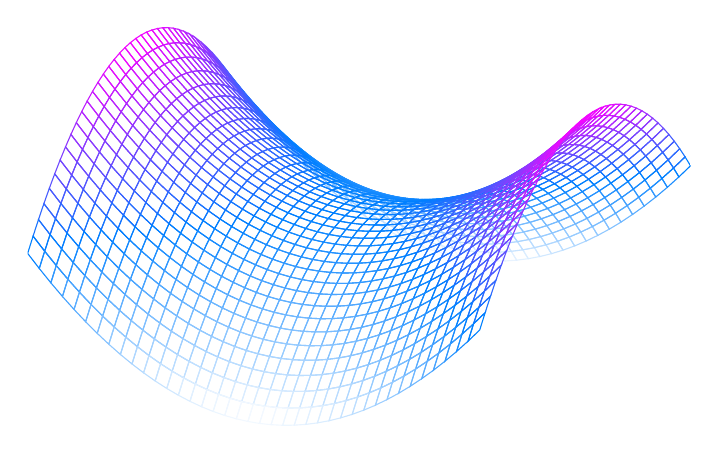
\begin{tikzpicture}\begin{axis}[hide axis,
xlabel=$x$,ylabel=$y$,colormap/cool, ]
\addplot3[domain=-3:3,mesh,samples=40]{x^2-y^2};
\end{axis}\end{tikzpicture}\end{center}
\newpage
\subfile{revisedsections/Introduction}
\newpage
\tableofcontents
\newpage
\section{Limits} \subfile{revisedsections/IntroToLimits}
\subsection{Types of Limits} \subfile{revisedsections/TypesOfLimits} 
\newchapter{Directly Calculating Limits}{DirectlyCalculatingLimits}
\newchapter{The Squeeze Theorem}{SqueezeTheorem}
\subsection{Relative Magnitudes} \subfile{revisedsections/RelativeMagnitudes}\newpage
\section{Derivatives} \subfile{revisedsections/IntroToDerivatives}
\newchapter{The Difference Quotient}{DifferenceQuotient}
\subsection{Estimating Derivatives}\subfile{revisedsections/EstimatingDerivatives}
\newchapter{Rules of Derivatives}{DerivativeRules}
\subsection{Implicit Differentiation}\subfile{revisedsections/ImplicitDifferentiation}\newpage
\subsection{Maxima and Minima} \subfile{revisedsections/MaxAndMin}
\subsection{Concavity} \subfile{revisedsections/Concavity}
\subsection{Graphical Relations} \subfile{revisedsections/DerivativeGraphs}
\subsection{Relationship with Continuity} \subfile{revisedsections/DerivativesAndContinuity}
\newpage
\section{Applications of Derivatives}
\subsection{Units}\subfile{revisedsections/DerivativeUnits}
\subsection{Instantaneous Rate of Change}\subfile{revisedsections/InstantaneousRateOfChange}
\subsection{Tangent Line Approximations}\subfile{revisedsections/TangentLineApproximations}
\subsection{Physics}\subfile{revisedsections/DerivativePhysics}
\subsection{Related Rates}\subfile{revisedsections/DerivativeRelatedRates}
\subsection{Optimization}\subfile{revisedsections/Optimization}
\subsection{Differential Equations}\subfile{revisedsections/DifferentialEquations}
\subsection{Slope Fields}\subfile{revisedsections/SlopeFields}\newpage
\subsection{Mean Value Theorem}\subfile{revisedsections/MeanValueTheorem}
\subsection{L'h\^{o}pital's Rule}\subfile{revisedsections/LhospitalsRule}
\newpage
\section{Antiderivatives and Definite Integrals}
\subsection{Antiderivatives}\subfile{revisedsections/Antiderivatives}
\subsection{Riemann Sums}\subfile{revisedsections/RiemannSums}
\subsection{Limits of Riemann Sums}\subfile{revisedsections/LimitsOfRiemannSums}
\subsection{Rules of Integrals}\subfile{revisedsections/RulesOfIntegrals}
\subsection{Average Value}\subfile{revisedsections/AverageValue}
\subsection{Integrals Generating Functions}\subfile{revisedsections/IntegralsGeneratingFunctions}
\subsection{Calculating Area}\subfile{revisedsections/CalculatingArea}
\subsection{Disc Method}\subfile{revisedsections/DiscMethod}
\subsection{Shell Method}\subfile{revisedsections/WasherMethod}
\newpage
\section{The Fundamental Theorem}
\subsection{Introduction}\subfile{revisedsections/FundamentalTheoremIntroduction}
\subsection{Consequences}\subfile{revisedsections/FunadamentalTheoremConsequences}
\newpage
\section{Applications of the Funadamental Theorem}
\subsection{Differential Equations}\subfile{revisedsections/SolvingDifferentialEquations}
\subsection{Accumulation and Net Change}\subfile{revisedsections/AccumulationAndNetChange}\newpage
\subsection{Physics}\subfile{revisedsections/SolvingPhysicsWithFundamentalTheorem}
\newline\vspace{2in}
\begin{center}
And that's the end of all the theory behind AP Calculus AB!
\end{center}
\newpage
\section{Endnotes}\subfile{revisedsections/Endnotes}
\end{document}
